\subsection{Zobrazení navrhovaných komentářů}
\label{subsec:implementation-display}

Navrhované komentáře jsou učiteli zobrazeny přímo v pohledu na zdrojový kód, analogicky ke standardním komentářům, které učitelé přidávají manuálně.
Pro vizuální odlišení jsou navrhované komentáře označeny červenou barvou pozadí, zatímco standardní komentáře jsou zobrazeny žlutou případně zelenou barvou.
Toto barevné rozlišení umožňuje učiteli okamžitě identifikovat, které komentáře pocházejí z automatické LLM analýzy a které vložil on sám nebo jiný pedagog.

Navrhované komentáře (viz \figref{fig:frontend-comment}) jsou viditelné výhradně učitelům, studenti je ve svém pohledu na odevzdání nevidí.
Studentovi se zobrazují pouze ty komentáře, které učitel explicitně přijal neboť po přijetí se navrhovaná komentář vloží jakoby jej vložil učitel sám manuálně, a tedy se zobrazuje i studentovi.
Tímto způsobem je zajištěno, že navrhované komentáře slouží pouze jako návrhy pro učitele, kteří mají kontrolu nad tím, které z nich budou studentovi zobrazeny, a které ne.
Navrhované komentáře tak mohou být využity i jako inspirace pro učitele.

\begin{figure}[ht]
    \centering
    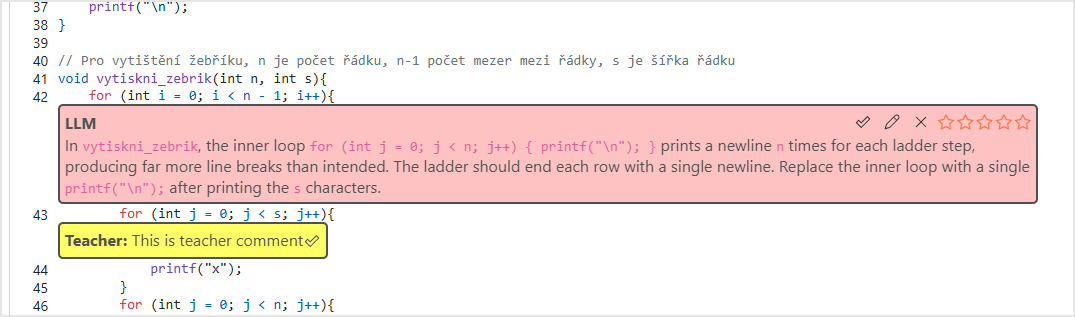
\includegraphics[width=1.0\textwidth]{resources/images/frontend-comment}
    \caption{Příklad zobrazení navrhovaných komentářů (červeně) a standardních komentářů (žlutě/zeleně) v pohledu učitele na zdrojový kód}
    \label{fig:frontend-comment}
\end{figure}

\endinput